\documentclass[letterpaper,12pt]{article}

\usepackage{rotating}
\usepackage[top=1in, bottom=1in, left=1in, right=1in]{geometry}
\usepackage{graphicx}
\usepackage[numbers,square,sort&compress]{natbib}
\usepackage{setspace}
\usepackage[cdot,mediumqspace,]{SIunits}
\usepackage{hyperref}

\begin{document}
\onehalfspacing
\title{Photon Counting and Statistics of Light}
\author{Anita Bahmanyar, Ayushi Singh, Carly Berard}
\date{30 September, 2013}

\maketitle
\begin{abstract}
\label{abstract}
Randomness is a phenomena that occurs often in the nature. Counting the number of photons would be one example of it. 

\end{abstract}


\section{Introduction}
\label{sec:introduction}
In this experiment, we will use the light detector device called Photomultiplier Tube, also known as PMT, in order to count the number of light particles(photons). The photometer consisted of PMT photon counting Head H10682, a counter and a computer which the PMT was connected to. The goal of this experiment is to show the randomness of the photons hitting the device and to show what the role of statistical methods in counting the photons is. Python programming language will be used to plot data and analyze them. Another aim of this lab would be to see what the limitations of detecting light is in astronomy.


\section{Experimental Procedure}
\label{sec:experimental procedure}
In order to take data, we first turned on PMT and ran its software on the main computer. Then, we used pmt.py python code to collect data. Afterwards, we wrote a small python code to  specify the sampling time and number of counts per second and finally we plotted the data, both normally and in histogram style. Figure 1 shows the normal and histogram graphs of counts versus time and figure 2 shows the histograms of the same data. These plots show the randomness of photon count, since none of the plots are the same. In order to get the count rate, one should divide the counts per sample by the sample time. For instance, here we could divide 100 by 0.001 to get the sample rate of 10000.

\begin{figure}[t]
\begin{center}
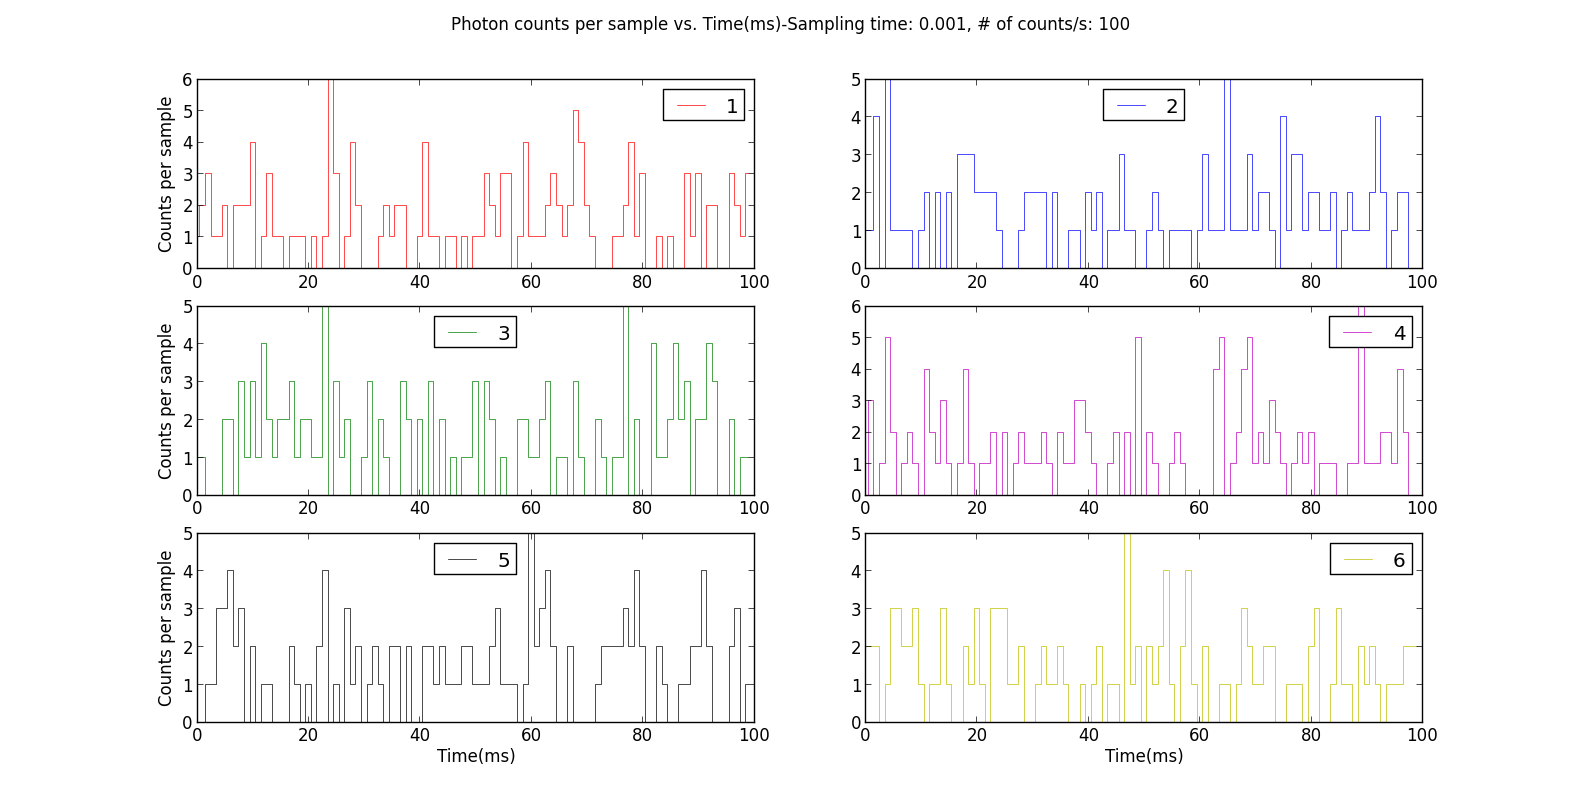
\includegraphics[scale=0.40]{ex_1_plot_1.png}
\caption{ Photon Count per Sample vs. Time plots}
The plots of number of counts versus time for sampling time of 0.001 and 100 photons per second. Six sets of data were taken with the same sampling time and count rate in order to show the randomness of the photon encounters. None of the plots are exactly the same; however, they have a similar overall shape.
\end{center}
\end{figure}


As we progressed, we wrote python codes to make life much easier for collecting data. What this code did was that it ran a loop that collected data and saved it under different names each time. Therefore, we ended up getting all the files organized and fast. I should also mention that Carly Berard mostly did the collection of data part and I should also give credit to Ayushi for collecting dark counts and some other parts throughout the lab.


\end{document}